%%%%%%%%%%%%%%%%%%%%%%%%%%%%%%%%%%%%%%%%%
% Beamer Presentation
% LaTeX Template
% Version 1.0 (10/11/12)
%
% This template has been downloaded from:
% http://www.LaTeXTemplates.com
%
% License:
% CC BY-NC-SA 3.0 (http://creativecommons.org/licenses/by-nc-sa/3.0/)
%
%%%%%%%%%%%%%%%%%%%%%%%%%%%%%%%%%%%%%%%%%

%----------------------------------------------------------------------------------------
%	PACKAGES AND THEMES
%----------------------------------------------------------------------------------------

\documentclass{beamer}

\mode<presentation> {

% The Beamer class comes with a number of default slide themes
% which change the colors and layouts of slides. Below this is a list
% of all the themes, uncomment each in turn to see what they look like.

%\usetheme{default}
%\usetheme{AnnArbor}
%\usetheme{Antibes}
%\usetheme{Bergen}
%\usetheme{Berkeley}
%\usetheme{Berlin}
%\usetheme{Boadilla}
%\usetheme{CambridgeUS}
%\usetheme{Copenhagen}
%\usetheme{Darmstadt}
%\usetheme{Dresden}
%\usetheme{Frankfurt}
%\usetheme{Goettingen}
%\usetheme{Hannover}
%\usetheme{Ilmenau}
%\usetheme{JuanLesPins}
%\usetheme{Luebeck}
\usetheme{Madrid}
%\usetheme{Malmoe}
%\usetheme{Marburg}
%\usetheme{Montpellier}
%\usetheme{PaloAlto}
%\usetheme{Pittsburgh}
%\usetheme{Rochester}
%\usetheme{Singapore}
%\usetheme{Szeged}
%\usetheme{Warsaw}

% As well as themes, the Beamer class has a number of color themes
% for any slide theme. Uncomment each of these in turn to see how it
% changes the colors of your current slide theme.

%\usecolortheme{albatross}
\usecolortheme{beaver} %nice
%\usecolortheme{beetle}
%\usecolortheme{crane} %nice
%\usecolortheme{dolphin} %nice
%\usecolortheme{dove}
%\usecolortheme{fly}
%\usecolortheme{lily} %nice
%\usecolortheme{orchid} %nice
%\usecolortheme{rose}
%\usecolortheme{seagull}
%\usecolortheme{seahorse}
%\usecolortheme{whale}
%\usecolortheme{wolverine}

%\setbeamertemplate{footline} % To remove the footer line in all slides uncomment this line
%\setbeamertemplate{footline}[page number] % To replace the footer line in all slides with a simple slide count uncomment this line

%\setbeamertemplate{navigation symbols}{} % To remove the navigation symbols from the bottom of all slides uncomment this line
}

\usepackage{graphicx} % Allows including images
\usepackage{booktabs} % Allows the use of \toprule, \midrule and \bottomrule in tables
\usepackage[belowskip=0pt,aboveskip=0pt]{caption}
\usepackage{amsmath}
\usepackage{pifont}
\usepackage{amsthm}
\usepackage{caption}
\usepackage[]{epstopdf}
\usepackage{braket}
\usepackage{color}
\usepackage{mathtools}

\usepackage{epsfig}
\usepackage{subfig}
\usepackage{float}
\usepackage{graphicx}


\usepackage{listings}
\lstdefinestyle{mystyle}{
%    backgroundcolor=\color{backcolour},   
%    commentstyle=\color{codegreen},
%    keywordstyle=\color{magenta},
%    numberstyle=\tiny\color{codegray},
%    stringstyle=\color{codepurple},
    basicstyle=\footnotesize,
    breakatwhitespace=false,         
    breaklines=true,                 
    captionpos=b,                    
    keepspaces=true,                 
    numbers=left,                    
    numbersep=5pt,                  
    showspaces=false,                
    showstringspaces=false,
    showtabs=false,                  
    tabsize=2
}
 
\lstset{style=mystyle}


\usepackage{caption}

\captionsetup[sub]{font=scriptsize,labelfont={}}

\providecommand{\abs}[1]{\lvert#1\rvert}


\usepackage{xcolor}
\definecolor{dgreen}{rgb}{0.,0.6,0.}
\definecolor{dred}{rgb}{1.,0.5,0.5}

\newcommand*{\Hhat}{\skew{5}{\hat}{H}}



%\setlength{\intextsep}{5pt plus 2pt minus 2pt}
%\setlength{\textfloatsep}{5pt plus 2pt minus 2pt}
%\setlength{\floatsep}{5pt plus 2pt minus 2pt}
\setbeamertemplate{frametitle}[default][center]
%----------------------------------------------------------------------------------------
%	TITLE PAGE
%----------------------------------------------------------------------------------------
\title[APPM 7400: HW\#1]{Hexagonal Grids for solving PDEs} % The short title appears at the bottom of every slide, the full title is only on the title page

\author[Prasanth Prahladan]{Prasanth Prahladan} % Your name
\institute[CU Boulder] % Your institution as it will appear on the bottom of every slide, may be shorthand to save space
{University of Colorado Boulder  \\ % Your institution for the title page
\medskip
%\textit{prasanth.prahladan@gmail.com} % Your email address
}
\date{\today} % Date, can be changed to a custom date

%\centering
%\titlegraphic{
%   \includegraphics[width=2cm]{Figures/iitm_logo.eps}
%}

\begin{document}
\scriptsize

\begin{frame}
\titlepage % Print the title page as the first slide
\end{frame}

%----------------------------------------------------------------------------------------
%	PRESENTATION SLIDES: 1
%----------------------------------------------------------------------------------------

\begin{frame}
\frametitle{Objectives}
\begin{enumerate}
\item Construction of Spatial Grid
\item Staggered Grids
\item Triangular and Hexagonal Nets
\item Grid functions for solving PDEs
\item Finite Difference Operators
\item Stability Conditions 
\item Numerical Dispersion
\item Example: Use of Staggered Grids in Computational Optics/Electro-magnetics
\end{enumerate}

\end{frame}


%----------------------------------------------------------------------------------------
%	PRESENTATION SLIDES
%----------------------------------------------------------------------------------------
\begin{frame}
\frametitle{Introduction to Spatial Grid}
\begin{figure}
%\vspace*{-1.5cm}
%\centering
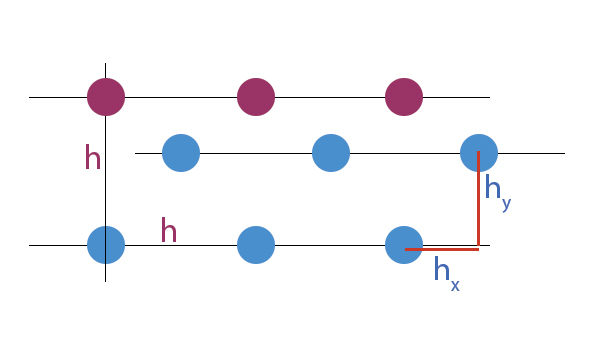
\includegraphics[scale=0.2]{./images/jpgSpatialGrid.jpg}
\label{fig:spatialGrid}
\end{figure}

A regular 2-D spatial grid is a collection of points defined as:
\begin{align*}
\mathbf{G}_h = \bigg\{\mathbf{r}_{m_1, m_2} = h \big( m_1 \mathbf{x_1} + m_2 \mathbf{x_2} \big) | (m_1,m_2) \in \mathbb{Z}^2\bigg\}
\end{align*}

A hexagonal grid is obtained when we displace each layer of points by $(h_x, h_y) = (\frac{h}{2}, \frac{h\sqrt{3}}{2})$.
\end{frame}

%----------------------------------------------------------------------------------------

\begin{frame}
\frametitle{Spatial Grids}

For each regular lattice, a suitable coordinate axis may be chosen for facilitating analysis. 
For the Rectilinear Grid, we have $\big( \mathbf{x_1}, \mathbf{x_2} \big) = \big([1,0]^T, [0,1]^T \big)$.
\begin{figure}
\centering
\begin{minipage}{.5\textwidth}
  \centering
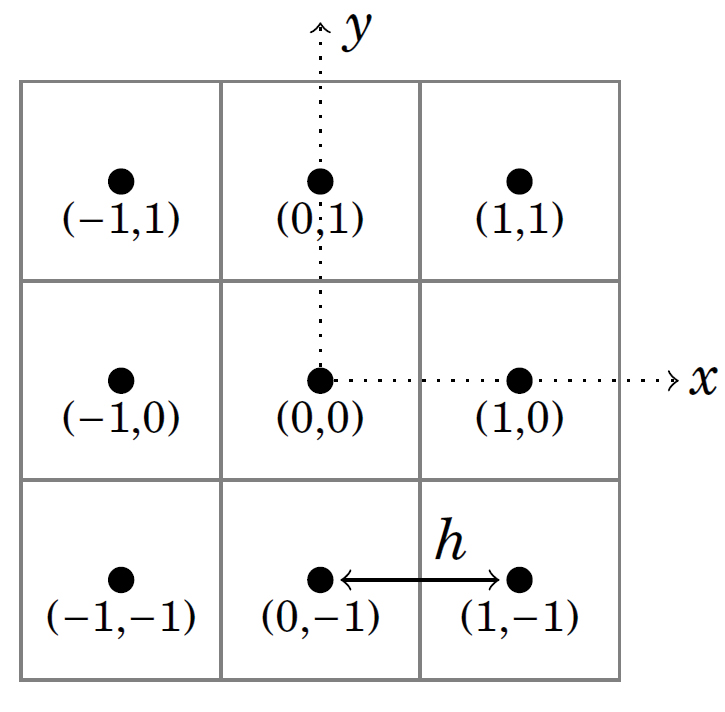
\includegraphics[scale=0.2]{./images/jpgRect.jpg}
\label{fig:RectilinearGrid}
\captionof{figure}{Rectilinear Grid}
\end{minipage}%
\begin{minipage}{.5\textwidth}
  \centering
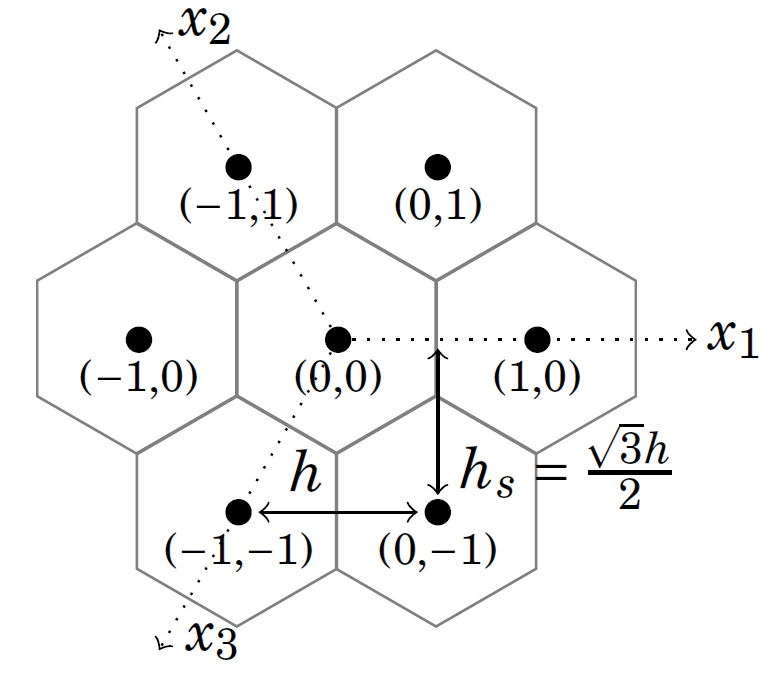
\includegraphics[scale=0.2]{./images/jpgHex.jpg}
\label{fig:HexGrid}\
\captionof{figure}{Hexagonal Grid}
\end{minipage}


\end{figure}

For the Hexagonal Grid, we have $\big( \mathbf{x_1}, \mathbf{x_2} \big) = \big([1,0]^T, [\frac{-1}{2},\frac{\sqrt{3}}{2}]^T \big)$.

\end{frame}

%----------------------------------------------------------------------------------------

\begin{frame}
\frametitle{Staggered Grids}

\begin{figure}
\centering
\begin{minipage}{.5\textwidth}
  \centering
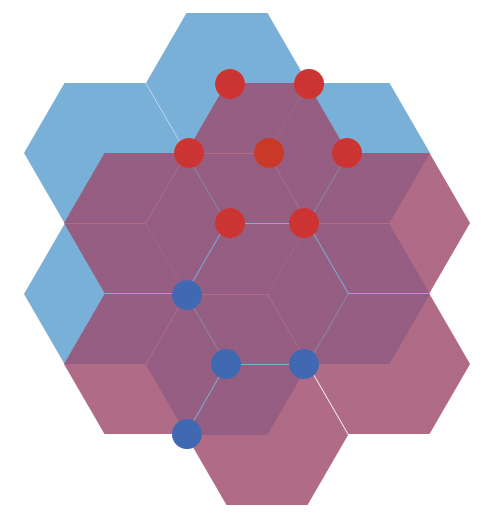
\includegraphics[scale=0.2]{./images/jpgStaggeredColocated.jpg}
\label{fig:StaggeredColocated}
  \captionof{figure}{Staggered Colocated Hexagonal Grids}
\end{minipage}%
\begin{minipage}{.5\textwidth}
  \centering
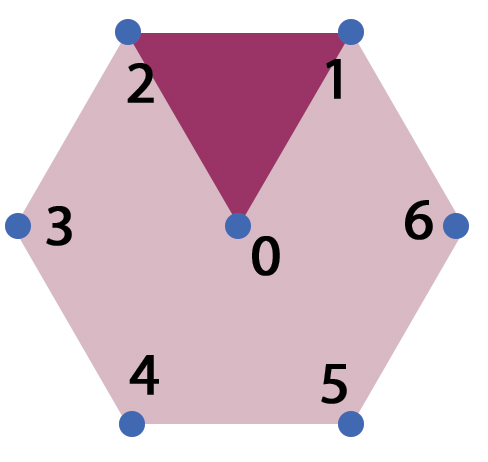
\includegraphics[scale=0.2]{./images/jpgHexGridStruc.jpg}
\label{fig:HexGridStructure}
\captionof{figure}{Hexagonal Grid Structure}
\end{minipage}
\end{figure}



\end{frame}

\begin{frame}

\begin{figure}
 \begin{center}
 \subfloat[]{
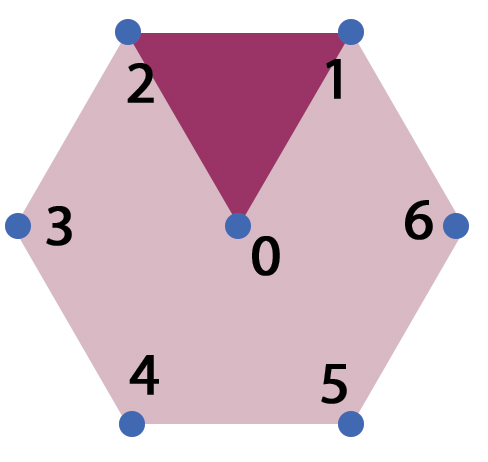
\includegraphics[scale=0.1]{./images/jpgHexGridStruc.jpg}
  }
  \quad
  \subfloat[]{
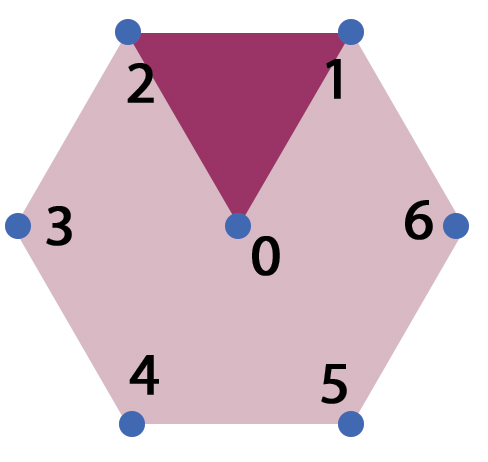
\includegraphics[scale=0.1]{./images/jpgHexGridStruc.jpg}
  }\quad
   \subfloat[]{
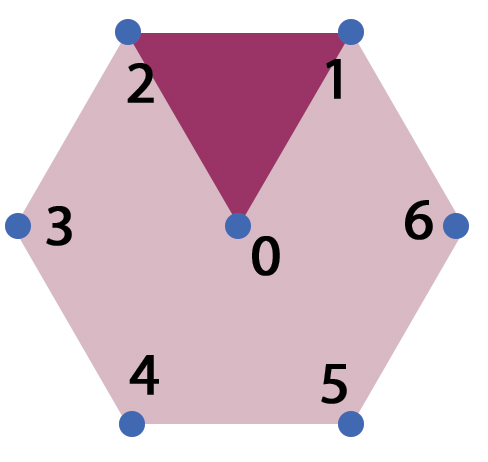
\includegraphics[scale=0.1]{./images/jpgHexGridStruc.jpg}
  }\\
  \subfloat[]{
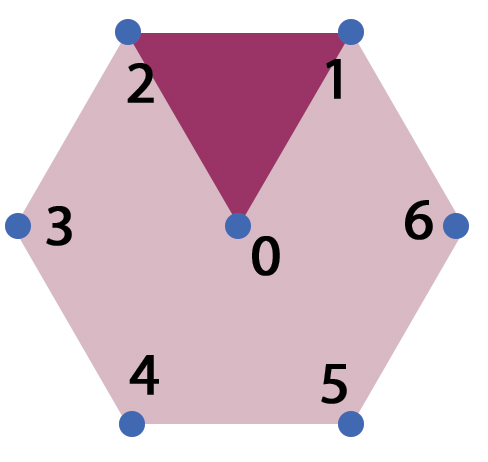
\includegraphics[scale=0.1]{./images/jpgHexGridStruc.jpg}
  }\quad
  \subfloat[]{
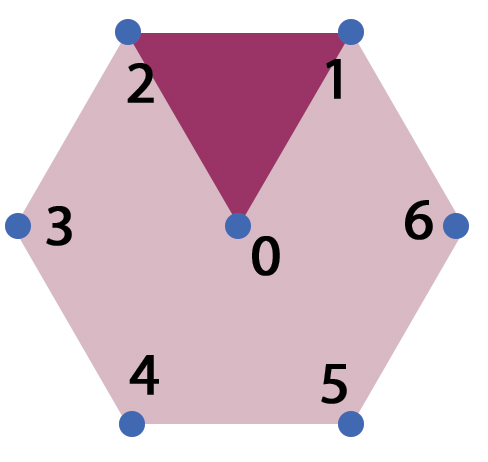
\includegraphics[scale=0.1]{./images/jpgHexGridStruc.jpg}
  }\quad
  \subfloat[]{
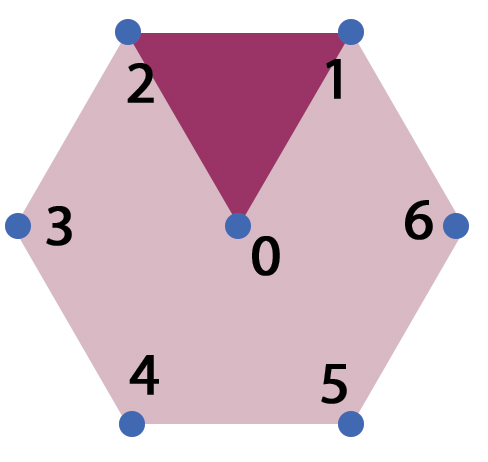
\includegraphics[scale=0.1]{./images/jpgHexGridStruc.jpg}
  }
  \caption{Including multiple Images with one caption}\vspace{-10mm}
  \label{fig:stab_chart}
  \end{center}
\end{figure}

\end{frame}



\begin{frame}
\frametitle{Triangular and Hexagonal Nets}
\tiny
\begin{minipage}{.5\textwidth}
  \centering
  Triangular Net
\begin{align*}
u_1 - u_0 &= u(x+h,y) - u(x,y) \\
&= h (\frac{\partial}{\partial x})u + \frac{h^2}{2!}(\frac{\partial^2 }{\partial^2 x})u + \frac{h^3}{3!} (\frac{\partial^3}{\partial^3 x})u + \cdots\\
u_2 - u_0 &= u(x+\frac{h}{2},y+\frac{\sqrt{3}h}{2}) - u(x,y) \\
&= h \bigg(\frac{1}{2}\frac{\partial}{\partial x} + \frac{\sqrt{3}}{2} \frac{\partial}{\partial y} \bigg)u \\
&+ \frac{h^2}{2!}\bigg(\frac{1}{2}\frac{\partial}{\partial x} + \frac{\sqrt{3}}{2} \frac{\partial}{\partial y} \bigg)^2 u \\
&+ \frac{h^3}{3!} \bigg(\frac{1}{2}\frac{\partial}{\partial x} + \frac{\sqrt{3}}{2} \frac{\partial}{\partial y} \bigg)^3 u + \cdots\\
u_3 - u_0 &= u(x-\frac{h}{2},y+\frac{\sqrt{3}h}{2}) - u(x,y) \\
&= h \bigg(\frac{-1}{2}\frac{\partial}{\partial x} + \frac{\sqrt{3}}{2} \frac{\partial}{\partial y} \bigg)u \\
&+ \frac{h^2}{2!}\bigg(\frac{-1}{2}\frac{\partial}{\partial x} + \frac{\sqrt{3}}{2} \frac{\partial}{\partial y} \bigg)^2 u \\
&+ \frac{h^3}{3!} \bigg(\frac{-1}{2}\frac{\partial}{\partial x} + \frac{\sqrt{3}}{2} \frac{\partial}{\partial y} \bigg)^3 u + \cdots\\
\cdots (u_4-u_0), &(u_5-u_0), (u_6-u_0)
\end{align*}
\end{minipage}%
\begin{minipage}{.5\textwidth}
  \centering
  Hexagonal Net
\begin{align*}
u_1 - u_0 &= u(x+\frac{h}{2},y+\frac{\sqrt{3}h}{2}) - u(x,y) \\
&= h \bigg(\frac{1}{2}\frac{\partial}{\partial x} + \frac{\sqrt{3}}{2} \frac{\partial}{\partial y} \bigg)u \\
&+ \frac{h^2}{2!}\bigg(\frac{1}{2}\frac{\partial}{\partial x} + \frac{\sqrt{3}}{2} \frac{\partial}{\partial y} \bigg)^2 u \\
&+ \frac{h^3}{3!} \bigg(\frac{1}{2}\frac{\partial}{\partial x} + \frac{\sqrt{3}}{2} \frac{\partial}{\partial y} \bigg)^3 u + \cdots\\
u_2 - u_0 &= u(x-h,y) - u(x,y) \\
&= -h (\frac{\partial}{\partial x})u + \frac{h^2}{2!}(\frac{\partial^2 }{\partial^2 x})u + \frac{-h^3}{3!} (\frac{\partial^3}{\partial^3 x})u + \cdots\\
u_3 - u_0 &= u(x+\frac{h}{2},y-\frac{\sqrt{3}h}{2}) - u(x,y) \\
&= h \bigg(\frac{1}{2}\frac{\partial}{\partial x} + \frac{-\sqrt{3}}{2} \frac{\partial}{\partial y} \bigg)u \\
&+ \frac{h^2}{2!}\bigg(\frac{1}{2}\frac{\partial}{\partial x} + \frac{-\sqrt{3}}{2} \frac{\partial}{\partial y} \bigg)^2 u \\
&+ \frac{h^3}{3!} \bigg(\frac{1}{2}\frac{\partial}{\partial x} + \frac{-\sqrt{3}}{2} \frac{\partial}{\partial y} \bigg)^3 u + \cdots\\
\end{align*}
\end{minipage}
\end{frame}


\begin{frame}
\frametitle{Triangular and Hexagonal Nets}
\tiny

\centering
\begin{minipage}{.5\textwidth}
  \centering
Triangular Net
% \sum_{i=1}^{6} u_i - 6 u_0 &= \frac{3h^2}{2!} \Delta u + \frac{(3/2 h^2)^2}{4} + \cdots \notag \\
\begin{align}
\frac{2}{3h^2}(\sum u_i - 6 u_0) &= \Delta u + \frac{h^2}{16} \Delta^2 u \notag \\
&+ R_0 \bigg(O(h^4)O\big( \frac{\partial^6}{\partial^k x \partial^{6-k}y}\big)\bigg)
\end{align}
\end{minipage}%
\begin{minipage}{.5\textwidth}
  \centering
Hexagonal Net
\begin{align}
\frac{4}{3h^2} \bigg( \sum_{i=1}^3 u_i - 3 u_0 \bigg) &= \Delta u \notag \\
&+ R_0 \bigg( O(h) O(\frac{\partial^3}{\partial^k x \partial^{3-k} y})\bigg)
\end{align}
\end{minipage}

\end{frame}



%----------------------------------------------------------------------------------------

\begin{frame}
\frametitle{Grid-functions for solving PDEs}

\begin{figure}
%\vspace*{-1.5cm}
%\centering
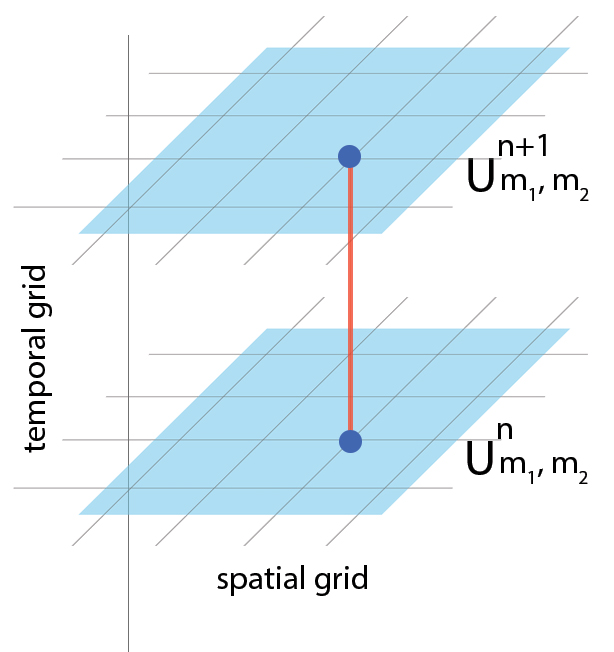
\includegraphics[scale=0.2]{./images/jpgGridFunction.jpg}
\label{fig:GridFunctions}
\end{figure}

We define a grid function $u^{n}_{m_1, m_2}$ as a time series at each point on the spatial grid which approximates the continuous functions $u(t,x,y)$ at time $t = nk$, where $k$ is the time-step and at the spatial position $(x,y)=\mathbf{r}_{m_1,m_2}$.

\end{frame}
%----------------------------------------------------------------------------------------

\begin{frame}
\frametitle{Finite Difference Operators}

In the FDTD method, differential operators are approximated by finite difference operators. 

First, we define the Unit-Shift operators as follows:
\begin{align}
S_{t\pm}\big( u^n_{m_1,m_2}\big) &= \big( u^{n+1}_{m_1,m_2}\big)\\
S_{x_1 \pm}\big( u^{n}_{m_1,m_2}\big) &= \big( u^{n}_{m_1 \pm 1,m_2}\big)\\
S_{x_2 \pm}\big( u^{n}_{m_1,m_2}\big) &= \big( u^{n}_{m_1,m_2 \pm 1}\big)\\
S_{x_3 \pm} &= S_{x_2 \mp} \cdot S_{x_2 \mp}
\end{align}

Next, we proceed to build second-order finite difference operators as:
\begin{align}
\delta_{tt} &= \frac{1}{k^2} \big( S_{t-} + S_{t+} -2 \big)\\
\delta_{x_i x_i} &= \frac{1}{h^2} \big( S_{x_i -} + S_{x_i +} -2 \big)\\
\end{align}
\end{frame}

\begin{frame}
\frametitle{Finite Difference Operators}
On the hexagonal grid we employ seven-points to build a second-order accurate approximation to the Laplacian:
\begin{align}
\delta_{\Delta \text{HEX}} &= \frac{2}{3} \big( \delta_{x_1 x_1} + \delta_{x_2 x_2} + \delta_{x_3 x_3}\big) \notag \\
&= \Delta + \frac{h^2}{16} \Delta^2 + O(h^4)
\end{align}
where $\Delta = \frac{2}{3}\big( \frac{\partial^2}{\partial x_1^2} + \frac{\partial^2}{\partial x_2^2} + \frac{\partial^2}{\partial x_3^2}\big)$ is the 2-D Laplacian operator for the 2-D Wave Equation
\begin{align}
\bigg(\frac{\partial^2}{\partial t^2} - c^2 \Delta \bigg) u = 0
\end{align}
\end{frame}
%----------------------------------------------------------------------------------------
\begin{frame}
\frametitle{Finite Difference Operators}
Using the finite-difference operators, we solve the approximate finite-difference 2-D Wave Equation
\begin{align}
\bigg(\frac{\partial^2}{\partial t^2} - c^2 \Delta \bigg) u^{n}_{m_1,m_2} = 0
\end{align}

using the explicit update equation
\begin{align}
u^{n+1}_{m_1,m_2} &= \frac{2\mu^2 }{3} \big( u^{n}_{m_1+1,m_2} + u^{n}_{m_1-1,m_2} + u^{n}_{m_1,m_2+1} \\
&+ u^{n}_{m_1,m_2-1} + u^{n}_{m_1+1,m_2+1} + u^{n}_{m_1-1,m_2-1} \big) \\
&+ (2-4\mu^2) u^{n}_{m_1,m_2} - u^{n-1}_{m_1,m_2}
\end{align}
where, 
\begin{align}
\mu = ck/h \label{eq:CourantNumber}
\end{align}
$\mu$ is the Courant Number, which is the ratio between the time step and the grid spacing for a given wave speed. 
\end{frame}



\begin{frame}
\frametitle{Stability Conditions}
\begin{figure}
\centering
\begin{minipage}{.5\textwidth}
  \centering
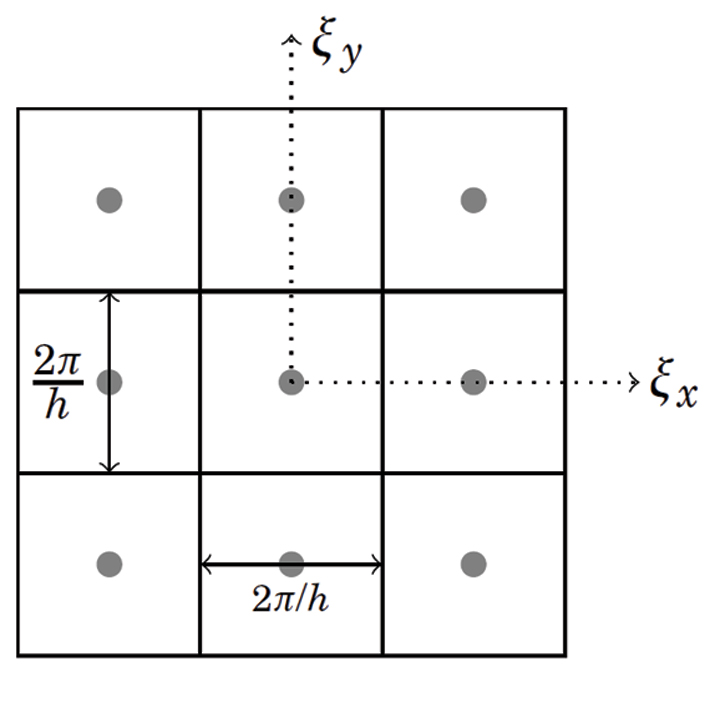
\includegraphics[scale=0.1]{./images/jpgDualRect.jpg}
\label{fig:DualRectGrid}
  \captionof{figure}{Dual-Rectilinear Grid}
\end{minipage}%
\begin{minipage}{.5\textwidth}
  \centering
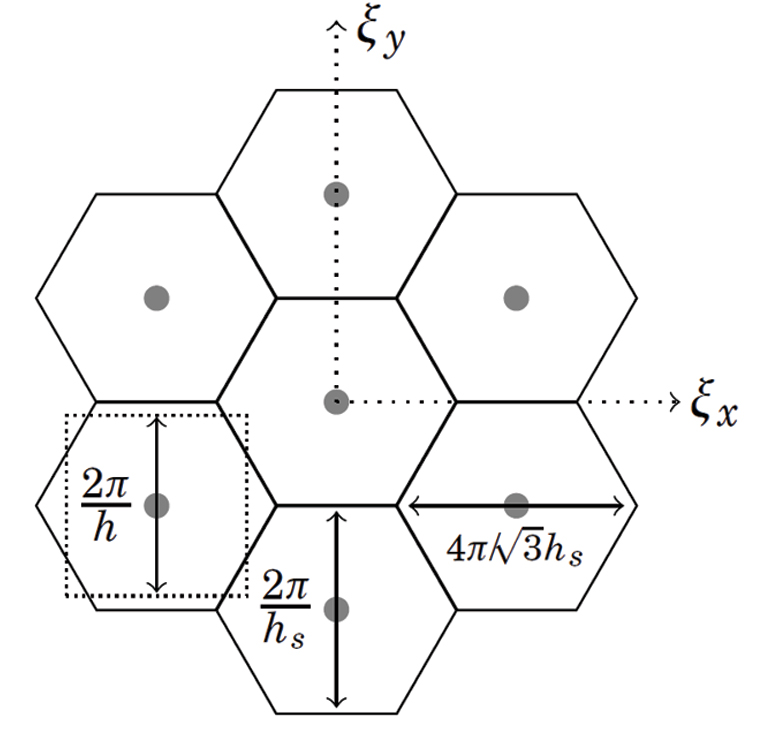
\includegraphics[scale=0.1]{./images/jpgDualHex.jpg}
\label{fig:DualHexGrid}
\captionof{figure}{Dual-Hexagonal Grid}
\end{minipage}
\end{figure}

Determine the maximum value of Courant Number, $\mu = ck/h$ such that no exponentially growing plane-wave solutions of the form
\begin{align*}
u^{n}_{m_1, m_2} = e^{jk n\omega } e^{jh (\xi_x, \xi_y)\cdot(m_1 \mathbf{x_1}+ m_2 \mathbf{x_2})}
\end{align*}
where $(\omega, \xi_x, \xi_y) \in \mathbb{C}^3$ are the wave-numbers in complex frequency domain, $(h,k) \in  \mathbb{R}^2$ grid spacing and the integral grid locations $(n,m_1,m_2) \in \mathbb{Z}^3$.

\end{frame}

\begin{frame}
\frametitle{Stability Conditions}

Stability Conditions:
\begin{enumerate}
\item $\omega \in [0,\pi]$
\item $(\xi_x, \xi_y) \in \{$ One Wave-Number Cell $\}$ of the Grid. 
\end{enumerate}


For the Hexagonal Grid, the maximum Courant number is determined to be 
\begin{align}
\mu \leq \sqrt{\frac{2}{3}}
\end{align}
which, is achieved at the corners of the hexagon. \\

By searching over $ \xi_x, \xi_y \in [-\frac{\pi}{h},\frac{\pi}{h}]$ is in-sufficient to cover the entire the hexagonal wave-number cell, due to issues with aliasing associated with Fourier analysis. The way the frequency ranges is handled not a trivial issue. 
\end{frame}

%----------------------------------------------------------------------------------------

\begin{frame}
\frametitle{Numerical Dispersion}

The condition for the plane waves of the form $u = e^{j\omega t} e^{j(\xi_x x + \xi_y y)}$ are solutions to the 2-D wave equation is given by the well-known dispersion relation
\begin{align}
\omega^2 = c^2 |\mathbf{\xi}|^2 = c^2 (\xi_x^2 + \xi_y^2) \label{eq:Dispersion}
\end{align}

The Phase Velocity(Wave Speed) for $|\mathbf{\xi}| > 0$ is $\omega / |\mathbf{\xi}| = c$.

The finite difference scheme approximates \eqref{eq:Dispersion} as
\begin{align}
\mathcal{D}_{tt}(\omega) = \mathcal{D}_{\Delta}(\mathbf{\xi}) \label{eq:DispersionFreqDomain}
\end{align}
for some $\mathcal{D}_{tt}: \mathbb{C} \rightarrow \mathbb{C}$ and $\mathcal{D}_{\Delta}: \mathbb{C}^2 \rightarrow \mathbb{C}$, which are Fourier symbols of the Finite-Difference Operators of the scheme. 
\begin{align}
\mathcal{D}_{tt}(\omega) &= -\frac{4}{k^2}sin^2\big(\omega \frac{k}{2}\big)\\
\mathcal{D}_{\Delta}(\mathbf{\xi}) &= -\frac{8}{3h^2} \sum_{i=1}^{3} sin^2\big((\mathbf{\xi}\cdot \mathbf{x_i})\frac{h}{2}\big)
\end{align}
\end{frame}


%----------------------------------------------------------------------------------------


\begin{frame}
\frametitle{Numerical Dispersion}
For all practical considerations, we consider Real-valued Frequencies and Wave-numbers.

To make $\mathcal{D}_{tt}$ injective, we consider the positive real wave-numbers $\xi \in \mathbb{B}$, where $\mathbb{B}$ is any Wave-Number Grid Cell.

If stability conditions are satisfied, we have
\begin{align}
\mathcal{D}_{tt}^{-1}\bigg( c^2 \mathcal{D}_{\Delta}(\mathbf{\xi})\bigg) : \mathbb{B}  \rightarrow \bigg[0, \frac{\pi}{k}\bigg]
\end{align}

Numerical Phase Velocity of as a function of wave-number:
\begin{align}
v(\mathbf{\xi}) = \frac{\omega(\mathbf{\xi})}{|\mathbf{\xi}|}, \omega(\mathbf{\xi}) = \mathcal{D}_{tt}^{-1}\bigg( c^2 \mathcal{D}_{\Delta}(\mathbf{\xi})\bigg).
\end{align}

Polar Plots: 
\begin{itemize}
\item Polar Radius: Temporal frequency $\omega$
\item Polar Angle: Angle of Propagation $\theta$ for $\mathbf{\xi} = (|\mathbf{\xi}|,\theta)$.
\end{itemize}

Numerical Phase Velocity(Wave-Speed) as a function of wave-number and temporal-frequency:
\begin{align*}
v\big(\omega(|\mathbf{\xi}|,\theta), \theta ) &= \frac{\omega(\mathbf{\xi})}{|\mathbf{\xi}|}, \text{ where }\\
\mathbf{\xi} = |\mathbf{\xi}|e^{j\theta}, \omega(\mathbf{\xi}) &= \mathcal{D}_{tt}^{-1}\bigg( c^2 \mathcal{D}_{\Delta}(\mathbf{\xi})\bigg)
\end{align*}

 
\end{frame}

\begin{frame}
\frametitle{Numerical Dispersion}

\begin{figure}
\centering
\begin{minipage}{.5\textwidth}
  \centering
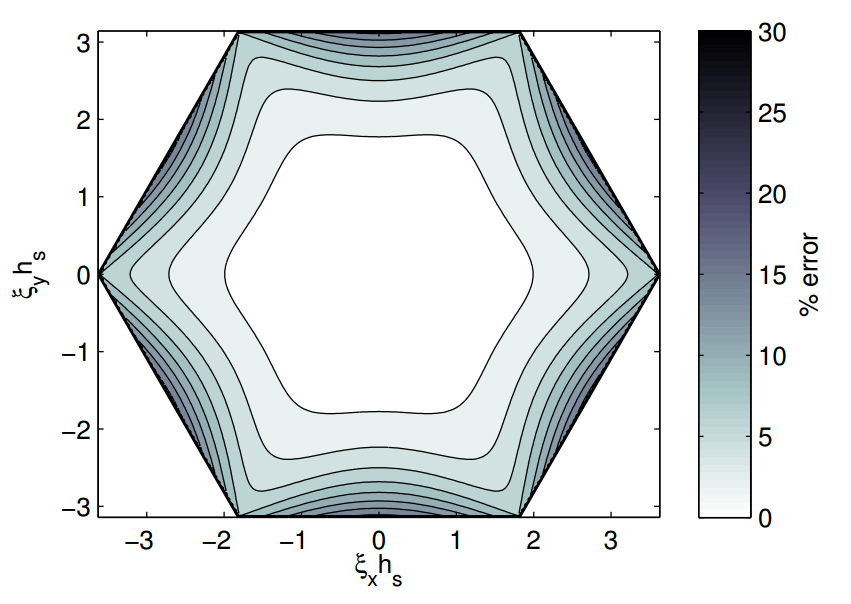
\includegraphics[scale=0.2]{./images/jpgVelocity.jpg}
\label{fig:NumericalDispersion}
  \captionof{figure}{Numerical Dispersion: Wave-number tiling}
\end{minipage}%
\begin{minipage}{.5\textwidth}
  \centering
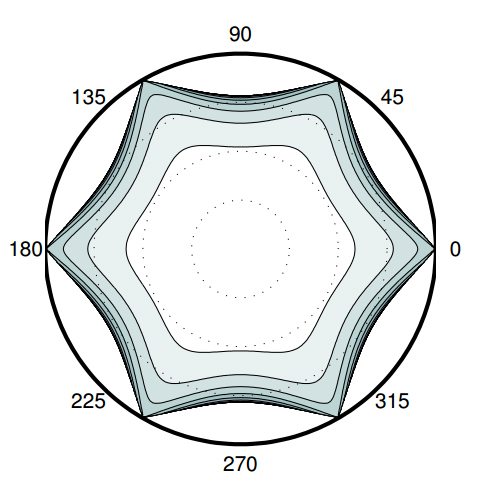
\includegraphics[scale=0.25]{./images/jpgVelocityPolar.jpg}
\label{fig:NumericalDispersionPolar}
\captionof{figure}{Numerical Phase Velocity: Polar plot}
\end{minipage}
\end{figure}



\end{frame}


%----------------------------------------------------------------------------------------

\begin{frame}
\frametitle{Application of Staggered Spatial Grids in Optics/Electro-magnetics}

\tiny

\begin{figure}
\centering
\begin{minipage}{.5\textwidth}
  \centering
\includegraphics[scale=0.2]{./images/jpgUnStaggered.jpg}
\label{fig:StaggeredColocated}
\end{minipage}%
\begin{minipage}{.5\textwidth}
  \centering
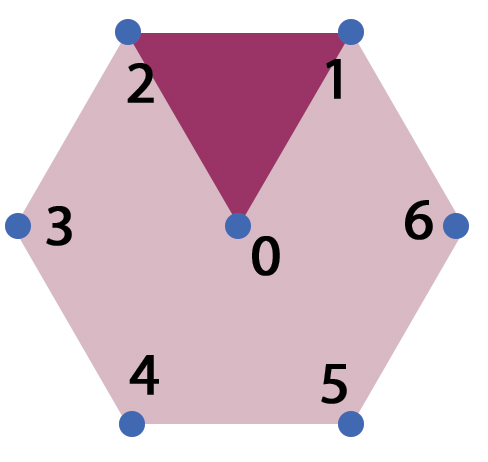
\includegraphics[scale=0.2]{./images/jpgHexGridStruc.jpg}
\end{minipage}
\end{figure}

\begin{minipage}{.5\textwidth}
  \centering
\begin{align*}
\frac{d D_{z0}}{dt} &= \frac{1}{6h}\bigg[ \big( 2 H_{y6} - 2 H_{y3} + H_{y1} - H_{y4} + H_{x5} - H_{x2} \big) \\
&- \sqrt{3}\big(H_{x1}- H_{x5} + H_{x2} - H_{x4}\big) \bigg]\\
\end{align*}
\end{minipage}%
\begin{minipage}{.5\textwidth}
  \centering
\begin{align*}
\frac{d B_{x0}}{dt} &= \frac{-\sqrt{3}}{6h} \big( E_{z1} - E_{z4} + E_{z2} - E_{z5}  \big)\\
\frac{d B_{y0}}{dt}&= \frac{1}{6h} \big( 2E_{z6} -2E_{z3} + E_{z1} - E_{z4} + E_{z2} - E_{z5}  \big)
\end{align*}
\end{minipage}
\end{frame}


\begin{frame}
\frametitle{Application of Staggered Spatial Grids in Optics/Electro-magnetics}
\tiny
\begin{figure}
\centering
\begin{minipage}{.5\textwidth}
  \centering
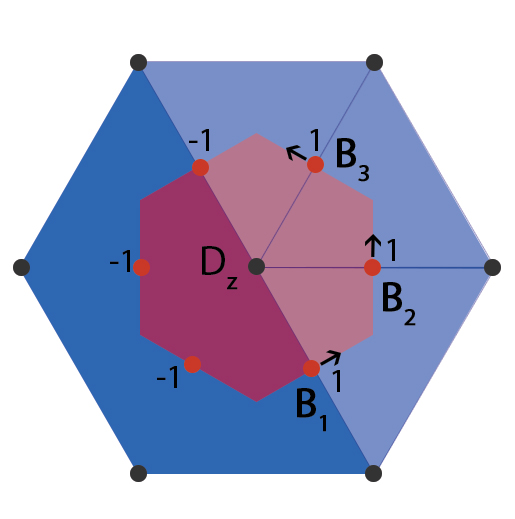
\includegraphics[scale=0.2]{./images/jpgStaggeredUncolocated.jpg}
\label{fig:StaggeredColocated}
\end{minipage}%
\begin{minipage}{.5\textwidth}
  \centering
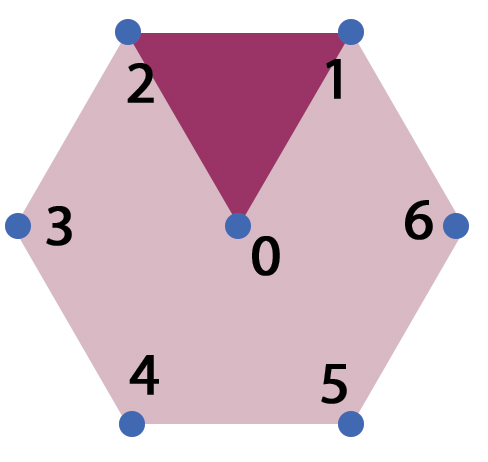
\includegraphics[scale=0.2]{./images/jpgHexGridStruc.jpg}
\end{minipage}
\end{figure}

\begin{minipage}{.5\textwidth}
  \centering
\begin{align*}
\frac{d D_{z0}}{dt} &= \frac{2}{3h} \big( H^a_1 - H^d_1 + H^b_2 - H^e_2 + H^c_3 - H^f_3 \big)\\
\frac{d B^a_1}{dt} &= \frac{1}{k} \big(E_{z5} - E_{z0} \big)\\
\end{align*}
\end{minipage}%
\begin{minipage}{.5\textwidth}
  \centering
\begin{align*}
\frac{d B^b_2}{dt}&= \frac{1}{k}\big( E_{z6} - E_{z0}\big)\\
\frac{d B^c_3}{dt}&= \frac{1}{k}\big( E_{z1} - E_{z0} \big)
\end{align*}
\end{minipage}

\end{frame}

%----------------------------------------------------------------------------------------
\begin{frame}
\frametitle{References}


\begin{thebibliography}{9}
\bibitem{yenliu}
Yen Liu,
  \emph{Fourier Analysis of Numerical Algorithms for the Maxwell Equations}.
Journal of Computational Physics 124, 396-416(1996)

\bibitem{brian}
Brian Hamilton and Stefan Bilbao,
\emph{Hexagonal vs. Rectilinear Grids for Explicit Finite Difference Schemes for the Two-Dimensional Wave Equation}
Proceedings of International Congress of Acoustics(ICA), Montreal, Canada(2013)

\bibitem{kantor}
Kantorovich and Krylov,
\emph{Approximate Methods of Higher Analysis} P Noordhoff Ltd., Groningen, Netherlands.(1964)

\bibitem{southwell}
R.V Southwell, \emph{Relaxation Methods in Theoretical Physics} Oxford University Press(1946)

\end{thebibliography}


\end{frame}




%----------------------------------------------------------------------------------------
%	PRESENTATION SLIDES : END
%----------------------------------------------------------------------------------------
\end{document}